\documentclass[../thesis/thesis.tex]{subfiles}
\renewcommand{\baselinestretch}{1.5}\selectfont
\graphicspath{{../figs/ch3-measunc/}}

\begin{document}
	
\onlyinsubfile{\setcounter{chapter}{2}}

\begin{refsection}
\chapter{Measurement Uncertainty}
\section{Introduction}

A measurement is an observation of a physical effect or quantity which provides useful information. This information, through the ages, has been used to facilitate advancement of both scientific knowledge and industrial development - from the production of standardised stone blocks to build the pyramids of ancient Egypt, to the production of standardised car parts to build Henry Ford's Model T. In the scientific realm, advanced measurement techniques at laboratories such as CERN are used to convince the world that new subatomic particles exist.

To communicate information about a measurement, the recipient needs to be able to either make or imagine a similar observation to that of the original measurer (or metrologist). The simplest way of doing this is to provide the recipient with the same physical effect or quantity for which to make their own observation (if you require a new nut for a bolt from a hardware shop, you might intuitively take the bolt with you), however, this can be inconvenient or impractical with larger objects, or if the recipient is located far away. Instead, you might substitute the physical effect or quantity with a more portable representation. For example, if you were to measure the size of a doorway to see if a new piece of furniture may fit through it, you might cut a piece of string to the same length and use this as the representation of the width of the item. However, this approach is very wasteful and also impractical for many physical effects (temperature, flow, pressure).

A solution widely thought to have been first established in the 3rd or 4th Millennium BC (see Figure \ref{ch3_fig_cubit}), is a system of units. In such a system, a discretised value of a quantity is standardised and knowledge of its value is disseminated to all people who wish to use it. Typically, a range of discrete values are chosen, such that the system of units can be conveniently used to represent all measurements. Knowledge of the discretised values is obtained from a primary standard which becomes the definition of the unit and is used to create copies of the standard which can be given to users of the unit system to perform measurements with. The most common method of performing measurements with a unit system is to use a standard to calibrate a measuring instrument, which can then be used to measure an arbitrary value of a quantity in the units defined by the standard.

\begin{figure}
	\centering
	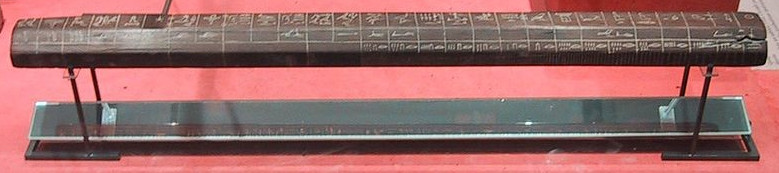
\includegraphics[width=\textwidth]{cubit}
	\caption{Egyptian royal cubit rod of Maya (treasurer of King Tutankhamun) 1336--1327 BC. The cubit is thought to be the earliest attested standard measure of length, first used in the 3rd or 4th Millennium BC.}
	\label{ch3_fig_cubit}
\end{figure}

The introduction of a regulated system of units enables commerce, as traded goods can be reliably valued between merchants across cities. This application is encountered by all citizens, and so there is a high demand for standards to be produced from the primary standard and physically distributed. It becomes impractical to create all standards by copying the primary standard directly (in some cases because the value of the primary standard is perturbed each time it is measured), and so a tiered organisational structure of standards is used. In this structure, there is a tier consisting of a small number of standards which are created directly from measurements of the primary standard, followed by subsequent tiers of larger numbers of standards which are derived from measurements of those in the previous tier. For any standard produced, it should be possible to trace the lineage back to a measurement of the primary standard. This is referred to as a traceability chain (see Figure \ref{ch3_fig_traceability}) and it is a fundamental tenet of metrology. Measurements with a shorter traceability chain are considered more traceable than those with longer chains.

\begin{figure}
	\centering
	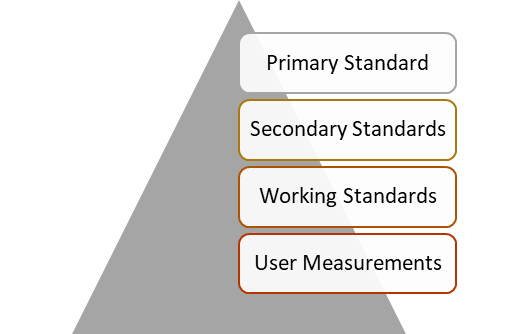
\includegraphics[]{traceability}
	\caption{The pyramid shows the number of instances in each tier. Secondary standards are held at NMIs and used to periodically calibrate working standards, which are sent by manufacturers and laboratories. User measurements are made using instruments calibrated with these working standards, so they number the greatest and are at the bottom of the traceability chain.}
	\label{ch3_fig_traceability}
\end{figure}

Today, the primary standards are maintained in most countries by a National Measurement Institute (NMI) and co-ordinated by the Bureau of International Weights and Measures (BIPM). To accommodate international trade and compatibility, a routine process of inter-comparisons is undertaken to ensure that the values of the primary standards between countries are in agreement.

Secondary standards are also kept by the NMIs and are used to reduce excessive wear to the primary standard caused by frequent measurements (and also to reduce bottlenecks caused by having a single standard). They are calibrated against the primary standard as infrequently as possible, again to reduce wear. Secondary standards are used by the NMI to characterise working standards which are sent to them by manufacturers and research institutes. Another important task of each NMI is to perform investigations to discover new and improved methods of measurement, which make use of secondary standards to better compare the accuracy of different methods.

Working standards are used, for example, by instrumentation manufacturers who may use them to calibrate their products before shipping to the customer, and more generally the standards can be used to calibrate test equipment to identify faulty products. Larger research institutes typically use working standards to recalibrate instrumentation prior to performing very sensitive measurements. To ensure that product specifications and scientific measurements are traceable and of high quality, accreditation services such as the United Kingdom Accreditation Service (UKAS) exist to certify manufacturers and laboratories that demonstrate good measurement practice and use traceable measurements \cite{UKAS}.

The selection of quantities for which primary standards are kept is only a subset of those for which recognised units exist. This is because many units are derived quantities, where their value can be obtained by calculation using definitions of other units. For example, the definition of the unit of resistance ($R$, ohms) can be derived from that of voltage ($V$, volts) and current ($I$, amperes), because $R=V/I$. The eight fundamental ``base'' units which make up the International System of Units (SI), are the metre, kilogram, second, ampere, kelvin, candela and mole. From these unit definitions, it is possible to define any other derived unit in use. NMIs will usually keep secondary standards of most derived quantities that users may wish to calibrate against, which are traceable to one or more primary standards of the base units. Although traditionally all primary standards were defined by physical artefacts (e.g. metallic weights, burning candles), these are being gradually replaced by definitions involving physical constants (e.g. Plank, Boltzmann), which do not degrade over time or use. The ``Ninth SI Units'' \cite{SI}, a proposition recently accepted by the BIPM, covers the redefinition of four of the SI units (the ampere, the kilogram, the kelvin and the mole) which will come into effect by May 2019.

The crucial effect of traceability on measurements is the confidence in their results. Measurements with poor traceability (longer chains) will produce results which are likely to be less accurate than those with better traceability (shorter chains). The reason for this is measurement uncertainty, which will now be explained.

It is impossible to know the true value of a quantity being measured as many undesirable physical effects typically occur during the measurement process. These effects contribute error (an unwanted perturbation) to the measured value, causing a reduction in accuracy (the deviation of the  measured value from the true value). Typical sources of error in measurement include thermal noise, imperfect calibration and drift of environmental conditions from those at which a measuring instrument was calibrated. In some cases, it is possible to quantify and correct for these errors, but there are often many sources (some of which contribute very small errors) which cannot be corrected for. This is because either the error cannot be quantified or the value of the error will change over the duration of the measurement process (random errors). Any source of error which cannot be removed from a measurement becomes a source of uncertainty, because the deviation of the measured value from the true value due to this source of error is uncertain. If it is possible to quantify the amount of uncertainty in a measurement, then a degree of confidence can be formed about its value.
If every measurement has an associated uncertainty in its value, then any measurement involving the results of previous measurements will include uncertainty contributions from both measurements. Measurements with good traceability involve fewer sources of uncertainty than those with poor traceability, leading to a higher degree of confidence in the former. It is because of this fact that NMIs strive to reduce the uncertainties in their primary standard definitions, which in turn reduces the uncertainty in all traceable measurements.

Because it is impossible to know the amount of error in a source of uncertainty, probability and statistical theories are used to instead describe the amount of uncertainty associated with it. By the nature of these theories there are often several methods which can be used to obtain a result, which sometimes provide different values. To ensure consistency and portability of uncertainty definitions, measurement guides were created in each industry and area of science, which specialised in processing the results of typical measurements. In addition, different guides were produced depending on the level of accuracy required - as more accurate measurements often require more effort to complete. Although this practice allowed suitable measurement comparisons within each field (e.g. chemistry, mechanical engineering), ambiguities still existed in uncertainty definitions between fields. To address this, a landmark document was published in 1993 by the International Organisation for Standardisation (ISO), the Guide to the Expression of Uncertainty in Measurement (GUM) \cite{GUM_1993}. This document was the work of representatives from seven international organisations: the BIPM, the International Organisation of Legal Metrology (OIML), the International Electrotechnical Commission (IEC), the ISO, the International Federation of Clinical Chemistry and Laboratory Medicine (IFCC), the International Union of Pure and Applied Chemistry (IUPAC), and the International Union of Pure and Applied Physics (IUPAP). The GUM, updated in 2008 \cite{GUM_2008}, is still used today as a reference for the evaluation of measurement uncertainty in many laboratories and industries across the world. The seven original organisations which wrote the GUM, together with the International Laboratory Accreditation Cooperation (ILAC, of which UKAS is a member), form the Joint Committee for Guides in Metrology (JCGM), who maintain the GUM and subsequent additional documents. These additional documents consist of the International Vocabulary of Metrology (VIM) \cite{VIM} and two supplements to the GUM \cite{GUM_S1,GUM_S2}: Supplement 1 covers the use of a Monte Carlo method [9] in uncertainty evaluation; Supplement 2 is used where more than one quantity is measured at the same time (multivariate).

Throughout this dissertation, the methodologies presented in the GUM will be used. The international authority of the guide, developed by seven international organisations (including the two global standardisation bodies IEC and ISO), gives strong motivation to use it as a basis for a framework to evaluate uncertainty in measurement.

This Chapter describes the evaluation of uncertainty prescribed in the GUM and highlights an inconsistency in the current version of the GUM and associated documents (which can have a profound effect on electromagnetic measurements).

\section{The Measurement Process}

In contrast to basic evaluations of uncertainty, where only repeat measurements of the quantity of interest are analysed, the GUM prescribes a more rigorous approach, which defines a mathematical model of the measurement process (measurement model) and propagates uncertainty through that model to the result (measurands). This allows any uncertainties from previous measurements, including those involving standards in the traceability chain, to be included in the result. The measurement model can be simple, such as measuring resistance using input quantities of voltage and current, or complicated and multivariate, requiring many input quantities and producing many output quantities. In some cases, the measurement model may not be known and can be defined as a black box, but this has certain limitations discussed later with Monte Carlo methods.

The GUM defines a process that is to be followed when evaluating uncertainty in measurement. It consists of the following steps:

\begin{enumerate}
	\item Modelling the measurement.
	\item Evaluating standard uncertainty of input quantities.
	\item Determining combined standard uncertainty of the measurands.
	\item Determining expanded uncertainty of the measurands.
\end{enumerate}

where standard uncertainty is an uncertainty expressed as a standard deviation and expanded uncertainty defines an interval encompassing a large fraction of the distribution of values that could reasonably be attributed to the measurand.

\subsection{Modelling the Measurement}

We can define a set of measurands $Y$ as a functional relationship depending on $N$ other input quantities $X_1, X_2, \dots, X_N$:

\begin{equation}
Y=f(X_1,X_2,\dots,X_N)
\end{equation}

The estimate of the measurands $\bar{y}$ can therefore be found by evaluating the model using the estimates of each input quantity $\bar{x}_1,\bar{x}_2,…,\bar{x}_N$:

\begin{equation}
\bar{y}=f(\bar{x}_1,\bar{x}_2,…,\bar{x}_N)
\end{equation}

Each input quantity can be an observation made during this measurement, a result from a previous measurement, or another source of information such as a datasheet or specification. An example of a measurement model could be for a temperature measurement, where the input quantities would include the value observed from the meter, the previously measured values of two calibration temperatures, and the assumed values of those calibration temperatures. Using this method, uncertainty from the calibration can be included in the evaluation. This is especially true for uncertainties caused by systematic errors, which do not vary during the measurement process, and cannot be evaluated purely by performing repeat measurements.

\subsection{Evaluating Standard Uncertainty of Input Quantities}

Sources of uncertainty in measurement can be divided into two categories: Category A uncertainty components are those that are evaluated using statistical analysis of a series of observations (i.e. repeats); Category B components are those that are evaluated using other means.

The GUM presents methods that include the use of both Bayesian and classical probabilistic methods to evaluate the uncertainty in the input quantities for a measurement model. In particular, classical methods \cite{Neyman_1937} are used for the treatment of Category A uncertainty components and Bayesian methods [11] are used for the treatment of Category B uncertainty components. An informative discussion on these types of method can be found in \cite{White_2016}. Since the publication of the GUM, some authors have stated (for example, in \cite{Kacker_2006,Kacker_2005,Kacker_2003,Bich_2014}) that this combination of different probabilistic methods (i.e., Bayesian and classical) represents an inconsistency in the GUM methodology for evaluating measurement uncertainty. The author has published a paper considering the effects of this inconsistency on electromagnetic wave measurements at radio frequencies \cite{Stant_2016}, which forms the basis for this section of the chapter.

The supplements to the GUM \cite{GUM_S1,GUM_S2} resolve the above-mentioned inconsistency by introducing a method for treating the Category A uncertainties that follows a Bayesian approach \cite{Elster_2007}. Therefore, the two supplements no longer contain the inconsistency found in the original GUM document. However, as a consequence of this change, there is now inconsistency between the method used to evaluate uncertainty described in the GUM and that described in the two supplements. In many situations, these different methods do not have a significant impact on the overall uncertainty that is evaluated. For situations where a considerable number of input quantities are observed simultaneously, the two different approaches can produce significantly different values of uncertainty. Such situations often occur in the area of high-frequency electromagnetic metrology, which is the topic of this dissertation.

\subsubsection{Category A Evaluation}

\paragraph{GUM Method}

The classical statistical technique \cite{Neyman_1937} applied to Category A uncertainties in the current GUM assigns a Gaussian probability distribution to a series of observations of a randomly varying input quantity, itself also represented by a Gaussian distribution. Therefore, after $n$ observations $x_1,x_2,\dots,x_n$, the best available estimate (arithmetic mean of measured values), $\bar{x}$, and standard deviation, $s$, of a randomly varying input quantity, $X$, is written as

\begin{align}
\bar{x} & =\frac{1}{n}\sum_{i=1}^{n}x_i,\\
s & =\sqrt{\frac{1}{n-1}\sum_{i=1}^{n}(x_i-\bar{x})^2}
\end{align}

respectively, where $x_i$ is the result of the $i$th observation. Importantly, a minimum of two observations must be made ($n=2$) in order for $\bar{x}$ and $s$ to be defined. The standard uncertainty of the best estimate of $X$, $u(\bar{x})_{\textrm{GUM}}$ can be found by dividing $s$ by the square root of the number of observations:

\begin{equation}
u(\bar{x})_{\textrm{GUM}}=\frac{s}{\sqrt{n}}
\label{ch3_eqn_ux_gum}
\end{equation}

If there are correlated (mutually dependent) input quantities present in the measurement model, the covariances of each pair of input quantities must also be calculated before the propagation stage of the uncertainty evaluation. Both the standard uncertainties and the covariances for $N$ input quantities can be represented in a symmetric ($N\times N$) matrix containing the variance of each quantity ($s^2$) along the diagonal and the covariance between $x_i$ and $x_j$ in the $i$, $j$th element. This is called the “uncertainty matrix” in the GUM and the “measurement covariance matrix” in the GUM Supplement 2. An example given in the GUM and described later in this chapter, demonstrates this scenario using the example of a simultaneous measurement of resistance and reactance with voltage, current and phase as correlated input quantities \cite[Example~H.2]{GUM_2008}. Once the uncertainties of the input quantities have been evaluated, they are propagated through the measurement model. This requires the sensitivities of the measurand to each input quantity to be calculated to at least a first order approximation. The estimates of the input quantities are used in the measurement model to obtain the estimate of the measurand. The variances and covariances of the input quantities are combined with the sensitivity coefficients in order to obtain the variance of the measurand. The combined standard uncertainty of the measurand is equal to the positive square root of this value. The result of the measurement is then presented as the measurand estimate and combined standard uncertainty. Alternatively, the uncertainty is expressed in terms of an expanded uncertainty which is derived directly from the combined standard uncertainty.

\paragraph{GUM Supplement Method}

Both GUM supplements (GUM-S1/S2) \cite{GUM_S1,GUM_S2} use a Bayesian approach \cite{Klauenberg_2012} to assign a probability density function (PDF) to describe all input quantities. This approach results in the choice of a $t$-distribution to characterize Category A input quantities, in contrast to the Gaussian distribution used in the GUM. Of particular relevance to this paper is the inclusion of the degrees-of-freedom parameter, $\nu$, in the definition of the standard uncertainty and covariances of a $t$-distribution. Whereas for the Gaussian distribution $\nu$ is used as a measure of reliability of the standard uncertainty, it is explicitly required when using the $t$-distribution in order to obtain the standard uncertainty, $u(\bar{x})_{\textrm{SUPP}}$:

\begin{equation}
u(\bar{x})_{\textrm{SUPP}} = \frac{s}{\sqrt{n}} \times \sqrt{\frac{\nu}{\nu-2}},
\label{ch3_eqn_ux_supp_multiv}
\end{equation}

where $\nu=n-N$, with $n$ being the number of observations and $N$ being the number of input quantities. In the GUM-S1 only a univariate $t$-distribution is offered, which represents $N=1$ input quantities. For this case (\ref{ch3_eqn_ux_supp_multiv}) can be rewritten as:

\begin{equation}
u(\bar{x})_{\textrm{SUPP}} = \frac{s}{\sqrt{n}} \times \sqrt{\frac{n-1}{n-3}}.
\label{ch3_eqn_ux_supp_univ}
\end{equation}

Equation \ref{ch3_eqn_ux_supp_univ} is undefined if $n$ is less than four. This effectively prevents the standard uncertainty from being calculated for a single input quantity according to the guidance given in the GUM-S1 (and the GUM-S2). The commercial ramifications of this condition are significant and are discussed later in this chapter. Figure \ref{ch3_fig_scaling_factor} illustrates the ratio between the standard uncertainty values calculated for different numbers of observations of a single Category A input quantity using the GUM and the GUM-S1/S2 approaches. It can be seen that when $n = 4$, $u(\bar{x})_{\textrm{SUPP}} = \sqrt{3} \times u(\bar{x})_{\textrm{GUM}}$, and as the number of observations increases the results from both approaches converge: If $n$ tends to infinity, the $t$-distribution tends towards a Gaussian distribution. However, most commercial laboratories would avoid making large numbers of measurements as this reduces the efficiency of the process.

\begin{figure}
	\centering
	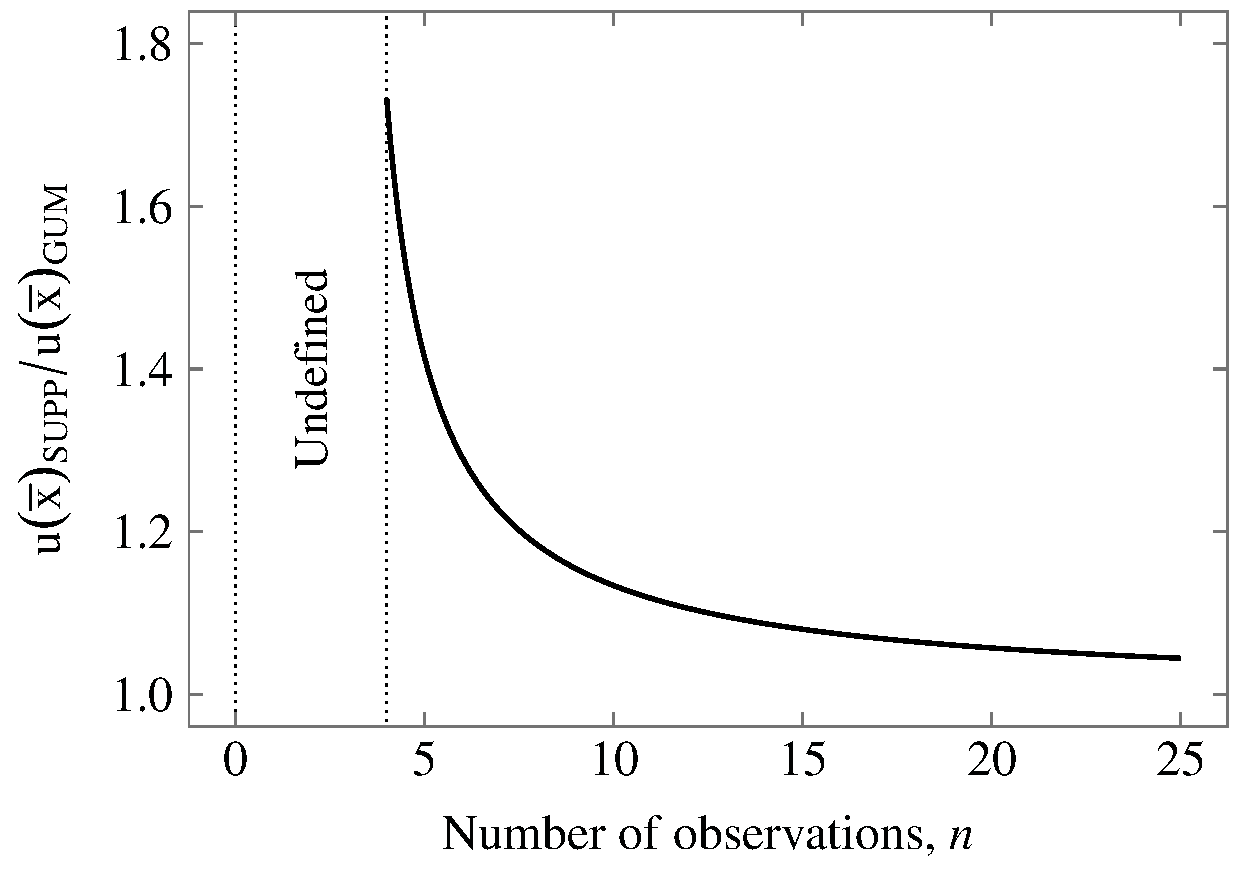
\includegraphics[width=0.65\textwidth]{scaling_factor}
	\caption{Scaling factor to convert from a GUM standard uncertainty to a GUM Supplement.}
	\label{ch3_fig_scaling_factor}
\end{figure}

For measurements involving multiple input quantities, such as the measurement of a vector quantity, a multivariate/joint distribution should be used as suggested in the GUM-S2. The variances and covariances between all pairs of input quantities are obtained using a matrix form of (\ref{ch3_eqn_ux_supp_multiv}) (\cite[Section~5.3.2]{GUM_S2}):

\begin{align}
\boldsymbol V(\boldsymbol X) & = \frac\nu{(\nu-2)}\frac{\boldsymbol S(\boldsymbol X)}n=\frac1{n(n-N-2)}\sum_{i=1}^n({\boldsymbol x}_i-\overline{\boldsymbol x}){({\boldsymbol x}_i-\overline{\boldsymbol x})}^\top
\\
\boldsymbol S(\boldsymbol X) & = \frac1\nu\hspace{0.35em}\sum_{i=1}^n({\boldsymbol x}_i-\overline{\boldsymbol x}){({\boldsymbol x}_i-\overline{\boldsymbol x})}^\top
\\
\boldsymbol V(\boldsymbol X) & = \begin{bmatrix}u{({\boldsymbol x}_1)}^2&u({\boldsymbol x}_1\text{,}{\boldsymbol x}_2)&\dots&u({\boldsymbol x}_1\text{,}{\boldsymbol x}_n)\\u({\boldsymbol x}_2\text{,}{\boldsymbol x}_1)&u{({\boldsymbol x}_2)}^2&\dots&u({\boldsymbol x}_2\text{,}{\boldsymbol x}_n)\\\vdots&\vdots&\ddots&\vdots\\u({\boldsymbol x}_n\text{,}{\boldsymbol x}_1)&u({\boldsymbol x}_n\text{,}{\boldsymbol x}_2)&\dots&u{({\boldsymbol x}_n)}^2\end{bmatrix}
\end{align}

where $\bm{U_X}$ is the uncertainty matrix, $\bm{x}_i$ is a sample from the array of vectors containing input quantity indications and $\bar{\bm{x}}$ is the arithmetic mean of that array. For this multivariate case, the minimum value of $n$ will increase linearly with $N$, such that the standard uncertainty is undefined unless $n > N + 2$. The consequences of this condition are demonstrated shortly.

\paragraph{Comparison of GUM and GUM Supplements approach using example H.2/9.4}

Both the GUM and the GUM-S2 provide an identical example which can be used to demonstrate the different standard uncertainties obtained when applying the method suggested in each document. The example is a simultaneous measurement of resistance and reactance, which uses a measurement model with multiple input quantities and multiple output quantities (measurands). The input quantities are voltage $V$, current, $I$, and phase, $\phi$, and the measurands are resistance $R$, reactance, $X$, and impedance, $Z$. The measurement model is defined as:

\begin{equation}
R=\frac VI\cos\theta, \quad X=\frac VI\sin\theta, \quad Z=\frac VI
\end{equation}

Six sets of indication values \cite{VIM} ($n = 6$) of $V$; $I$; $\phi$ are obtained independently by measurement. The version of this example given in the GUM uses only $n = 5$ sets, but one additional set of values of $V$; $I$; $\phi$ has been added for the GUM-S2 example to allow (\ref{ch3_eqn_ux_supp_multiv}) to be defined for $N = 3$ input quantities, a condition which was explained at the end of the previous section. These values, together with their arithmetic means and standard uncertainties as calculated from the two approaches using (\ref{ch3_eqn_ux_gum}) and the matrix form of (\ref{ch3_eqn_ux_supp_multiv}) (which is applicable to measurements involving multiple input quantities), are presented in Table \ref{ch3_tbl_gum_example}. The ratios of the standard uncertainties from each approach is also included in the table, which are identical for all these input quantities due to their dependence only on $n$ and $N$, which are also equal for all these input quantities (e.g. when $n = 6$ and $N = 3$, $\sqrt{(\nu/(\nu-2))}=\sqrt{((n-N)/(n-N-2))}=\sqrt{3}$. This explains why standard uncertainties evaluated with Category A methods using the minimum number of observations following the GUM-S1/S2 approach are always 1.732 times larger than the standard uncertainties calculated following the GUM approach.

\begin{table}[]
	\begin{tabular}{llll}
		Value             & $V$/V  & $I$/A   & $\phi$/rad   \\ \hline
		$x_1$             & 5.007  & 19.663  & 1.0456  \\
		$x_2$             & 4.994  & 19.639  & 1.0438  \\
		$x_3$             & 5.005  & 19.640  & 1.0468  \\
		$x_4$             & 4.990  & 19.685  & 1.0428  \\
		$x_5$             & 4.999  & 19.678  & 1.0433  \\
		$x_6$             & 4.999  & 19.661  & 1.0445  \\ \hline
		$\bar{x}$         & 4.9990 & 19.6610 & 1.04446 \\ \hline
		$u(\bar{x})\textrm{GUM}$   & 0.0026 & 0.0077  & 0.00061 \\
		$u(\bar{x})\textrm{SUPP}$  & 0.0045 & 0.0134  & 0.0011  \\ \hline
		$\frac {u(\bar{x})\textrm{GUM}}{u(\bar{x})\textrm{SUPP}}$ & 1.732  & 1.732   & 1.732  
	\end{tabular}
\caption{The indication values from the example ``Simultaneous Resistance and Reactance Measurement'' and their statistical properties as evaluated by the approaches given in \cite[Example H.2]{GUM_2008} and \cite[Example 9.4]{GUM_S2}.}
\label{ch3_tbl_gum_example}
\end{table}

\subsubsection{Category B Evaluation}
\subsection{Evaluating Combined Standard Uncertainty}
\subsubsection{Monte Carlo Methods}
\subsubsection{Law of Propagation of Uncertainty}
\subsubsection{Finite Difference Methods}
\subsection{Expanded Uncertainty and Coverage Intervals}
\section{Sensitivity Analysis}
\section{Conclusions}
\addcontentsline{toc}{section}{Bibliography}
\printbibliography
\end{refsection}
\end{document}
